\documentclass{llncs}

\usepackage{graphicx}
%\usepackage{algorithm2e}
%\usepackage{tabularx}
%\usepackage{url}
%\usepackage{subfigure}
%\usepackage{afterpage}
%\usepackage{amsmath,amssymb}            
%\usepackage{rotating}  
%\usepackage{fancyhdr}  
%\usepackage[scriptsize]{caption} 
%
\begin{document}
\title{Tampering detection for low-power smart camera}

\author{Author 1, Author 2}

\institute{Politecnico di Milano}
\maketitle

\begin{abstract}
	
	Abstract is here.
	
\end{abstract}

\section{Introduction}\label{sec:introduction}

Introduction is here.

\section{Related works}\label{sec:relWorks}

Other sections are here. 

\section{Problem formulation}\label{sec:probForm}

\section{Proposed solution}\label{sec:propSol}

\section{Experiments}\label{sec:experiments}
\begin{figure}
\centering
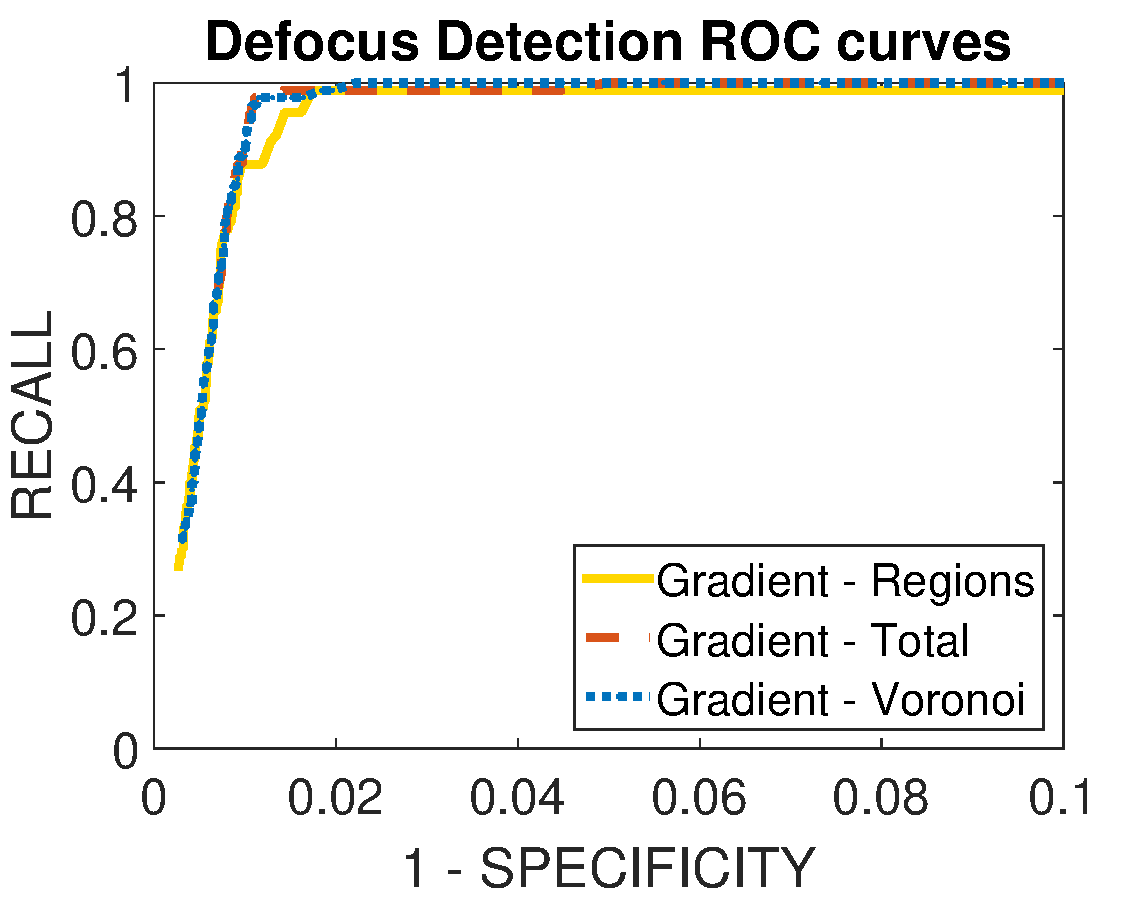
\includegraphics[width=0.7\linewidth]{Immagini/ROCdefocus_cropped.pdf}
\caption{Defocus}
\label{fig:ROCdefocus}
\end{figure}


\section{Conclusion}\label{sec:Conclusion}

Conclusions are here \cite{aksay2007camera}.

\section*{Acknowledgments}\label{sec:Acknowledgments}

Authors would like to thank YYYYY.

\bibliographystyle{unsrt}
\bibliography{bibl_tesi}

%\begin{thebibliography}{1}
%	
%	\bibitem{Einstein}
%	A. Einstein, On the movement of small particles suspended in stationary liquids required by the molecular-kinetic theory of heat, Annalen der Physik 17, pp. 549-560, 1905.
%	
%\end{thebibliography}
\end{document}
